% {{{ Preamble ----------------------------------------------------------------
\documentclass{beamer}

% encodings, fonts etc.
\usepackage[utf8x]{inputenc}
\usepackage[T1]{fontenc}

% Hold kæft utf
\makeatletter
\def\UTFviii@defined#1{%
  \ifx#1\relax
      ?%
  \else\expandafter
    #1%
  \fi
}

\makeatother

% math packages
\usepackage{amsmath, amssymb, amsthm}
\usepackage{mathtools}

% beamer configuration
\usetheme{Copenhagen}
%\useoutertheme{infolines}
%\usetheme{metropolis}
\beamertemplatenavigationsymbolsempty
%\setbeamertemplate{theorems}[numbered]
\setbeamersize{description width=2.0em}

%\usepackage{pgfpages}
%\setbeameroption{show notes}
%\setbeameroption{show notes on second screen=right}

% algorithms
\usepackage{algorithm}
\usepackage[noend]{algpseudocode}

% misc. packages
\usepackage{float}
\usepackage{varwidth}
\usepackage{listings}
\lstset{
  %breaklines=true,
  keepspaces=true,
  %frame=ltrb,
  %framesep=1pt,
  %commentstyle=\color{grey},
  basicstyle=\ttfamily\tiny,
  %numbers=left,
  title=\lstname,
  %columns=fullflexible,
  inputencoding=utf8,
  extendedchars=true,
}

% graphics and tikz
\usepackage{pgf}
\usepackage{tikz}
\usetikzlibrary{positioning,arrows,calc}
\tikzset{
    on grid,
    node distance=3cm,
    auto,
    block/.style = {
        draw,
        shape=rectangle,
        minimum height=3em,
        minimum width=3em,
        line width=1pt
    },
    control/.style = {
        draw,
        shape=circle,
        minimum height=7em,
        minimum width=3em,
        line width=1pt
    },
    mux/.style = {
        draw,
        shape=rectangle,
        minimum height=1.5em,
        minimum width=1em,
        line width=1pt
    },
    empty/.style = {
        shape=rectangle,
        minimum height=3em,
        minimum width=3em
    },
    >=latex',
}


% mathematics
\newtheorem{proposition}{Proposition}

\renewcommand{\tt}{\texttt}

% title page
\title{Pipelined MIPS processor}
\author[Carl-Johannes Johnsen]{
  \mbox{Carl-Johannes Johnsen}}
\institute{Department of Computer Science\\
           University of Copenhagen}
%\date{December 22, 2016}
% }}} -------------------------------------------------------------------------

\begin{document}

% {{{ Title page --------------------------------------------------------------
\frame{\titlepage}
% }}} -------------------------------------------------------------------------

% {{{ Table of contents -------------------------------------------------------
%\begin{frame}
%  \frametitle{Outline}
%  \tableofcontents
%\end{frame}
% }}} -------------------------------------------------------------------------
\section{Introduction}
\subsection{Overview}
\begin{frame}
    In this lecture, we will be looking at pipelining our single cycle MIPS
    processor.

    \vspace{\baselineskip}
    We will go through the motivation and background for pipelining, and the
    steps for implementing it in SME.

    \vspace{\baselineskip}
    Finally, we will look at handling the problems introduced by pipelining, by
    adding two new units: the Forwarding Unit, and the Hazard Detection Unit.
\end{frame}

\subsection{Motivation \& Background}
\begin{frame}
    The single cycle MIPS processor is not very efficient, as the clock rate is
    determined by the longest possible path in the processor.

    \vspace{\baselineskip}
    In order to increase the clock rate, we must decrease the longest path in
    the processor, by introducing pipes.
\end{frame}
\begin{frame}
    Pipes are registers in the processor, which temporarely store all the
    values computed so far.

    \vspace{\baselineskip}
    This ensures that the data does not have to travel as far, until it has
    reached a safe state.
\end{frame}
\begin{frame}
    Determining where to place the pipes, is done by dividing the processor
    into stages.

    \vspace{\baselineskip}
    We will follow the classic MIPS example, and divide the processor into 5
    stages:
    \begin{itemize}
        \item Instruction Fetch (IF)
        \item Instruction Decode (ID)
        \item Execute (EX)
        \item Memory (MEM)
        \item Write Back (WB)
    \end{itemize}
    We are going to insert a pipe between each state, i.e. 4 pipes.
\end{frame}
\begin{frame}
    \begin{figure}
        \centering
        \scalebox{0.5}{
            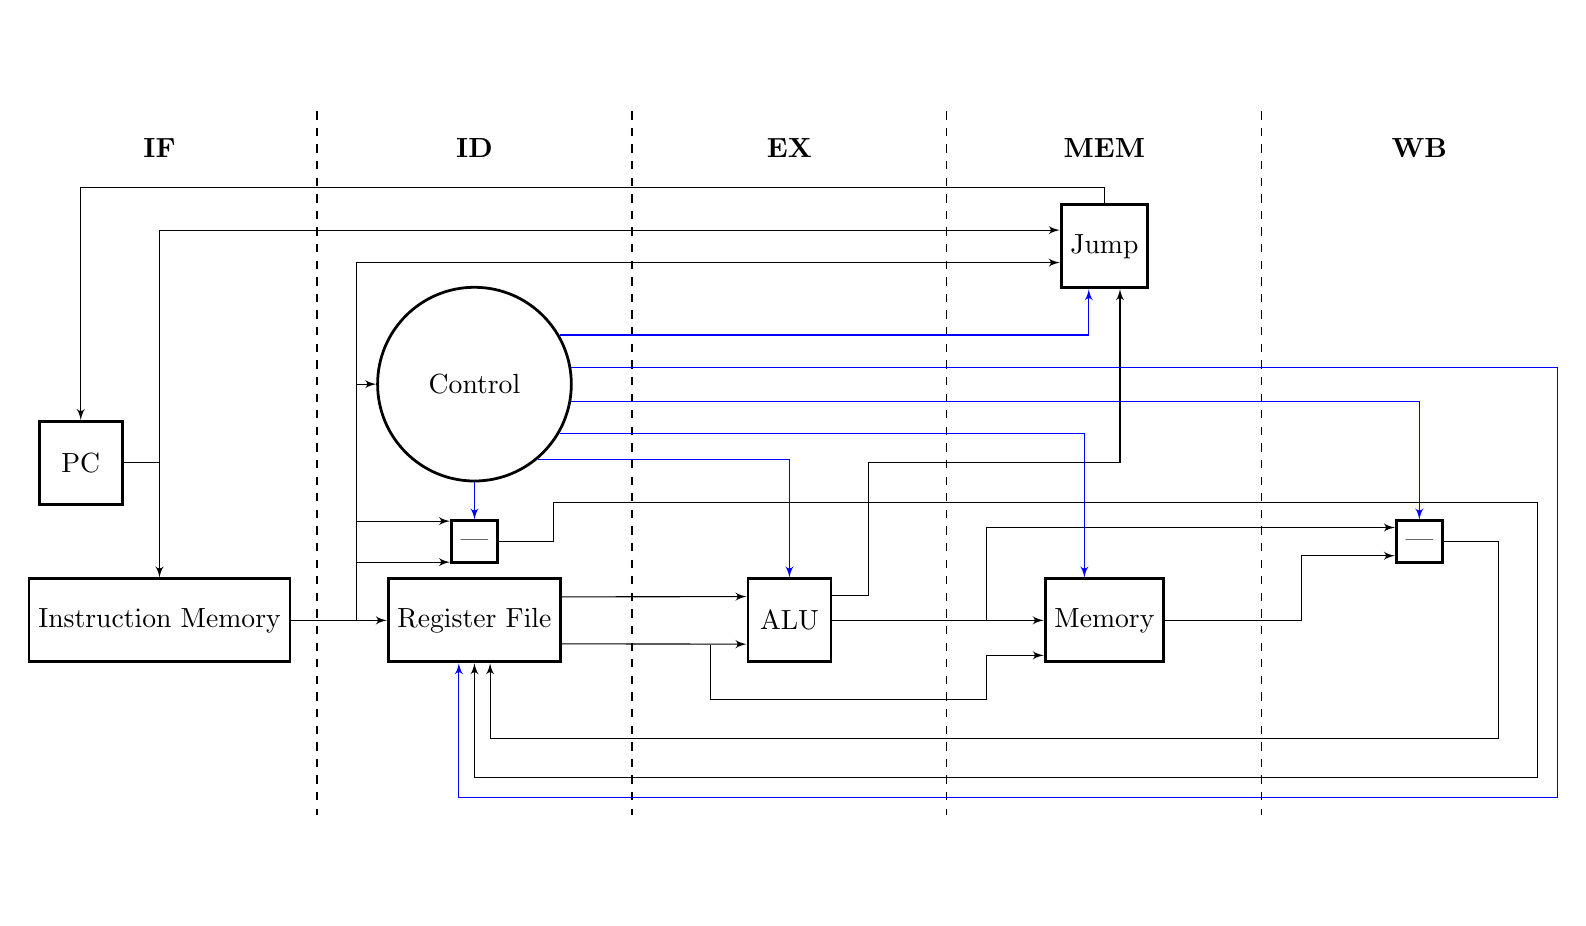
\begin{tikzpicture}
                \node[block] (alu) at (0,0) {ALU};
                \node[block] (reg) at (-4,0) {Register File};
                \node[block] (memo) at (4,0) {Memory};
                \node[block] (jump) at (4,4.75) {Jump};
                \node[block] (imem) at (-8,0) {Instruction Memory};
                \node[block] (pc) at (-9, 2) {PC};
                \node[control] (cont) at (-4, 3) {Control};
                \node[mux] (wbm) at (8,1) {|};
                \node[mux] (addr) at (-4, 1) {|};

                \node[empty] (if) at (-8, 6) {\textbf{IF}};
                \node[empty] (id) at (-4, 6) {\textbf{ID}};
                \node[empty] (ex) at (0, 6) {\textbf{EX}};
                \node[empty] (mem) at (4, 6) {\textbf{MEM}};
                \node[empty] (wb) at (8, 6) {\textbf{WB}};

                \node[empty] (ifidt) at (-6,7) {};
                \node[empty] (idext) at (-2,7) {};
                \node[empty] (exmemt) at (2,7) {};
                \node[empty] (memwbt) at (6,7) {};
                \node[empty] (ifidb) at (-6,-3) {};
                \node[empty] (idexb) at (-2,-3) {};
                \node[empty] (exmemb) at (2,-3) {};
                \node[empty] (memwbb) at (6,-3) {};

                \path[draw, dashed, -] (ifidt) -- (ifidb);
                \path[draw, dashed, -] (idext) -- (idexb);
                \path[draw, dashed, -] (exmemt) -- (exmemb);
                \path[draw, dashed, -] (memwbt) -- (memwbb);

                \path[draw, ->] (-5.5,0) |- (addr.220);
                \path[draw, ->] (-5.5,0) |- (addr.140);
                \path[draw, ->] (pc) -| (imem);
                \path[draw, ->] (imem) -- (reg);
                \path[draw, ->] (-5.5,0) |- (cont);
                \path[draw, ->] (reg.15) -- (alu.151);
                \path[draw, ->] (reg.345) -- (alu.209);
                \path[draw, ->] (alu) -- (memo);
                \path[draw, ->] (-1,-0.31) -| (-1,-1) -- (2.5,-1) |- (memo.210);
                \path[draw, ->] (2.5, 0) |- (wbm.150);
                \path[draw, ->] (memo) -- (6.5, 0) |- (wbm.210);
                \path[draw, ->] (wbm) -| (9, -1.5) -| (reg.290);
                \path[draw, ->] (alu.30) -| (1,1) |- (4,2) -| (jump.290);
                \path[draw, ->] (jump) |- (0,5.5) -| (pc);
                \path[draw, ->] (-8,2) |- (jump.160);
                \path[draw, ->] (-5.5,3) |- (jump.200);
                \path[draw, ->] (addr) -| (-3, 1.5) -| (9.5,-2) -|
                (reg.270);

                %\path[draw, color=blue, ->] (cont) -- (reg);
                %\path[draw, color=blue, ->] (cont.10) -| (9.5,-2) -| (reg.250);
                \path[draw, color=blue, ->] (cont.10) -| (9.75,-2.25) -| (reg.250);
                \path[draw, color=blue, ->] (cont.310) -| (alu);
                \path[draw, color=blue, ->] (cont.330) -| (memo.115);
                \path[draw, color=blue, ->] (cont.350) -| (wbm);
                \path[draw, color=blue, ->] (cont.30) -| (jump.250);
                \path[draw, color=blue, ->] (cont) -- (addr);
            \end{tikzpicture}
        }
        \label{fig:stages}
    \end{figure}
\end{frame}
\begin{frame}
    \begin{figure}
        \centering
        \scalebox{0.5}{
            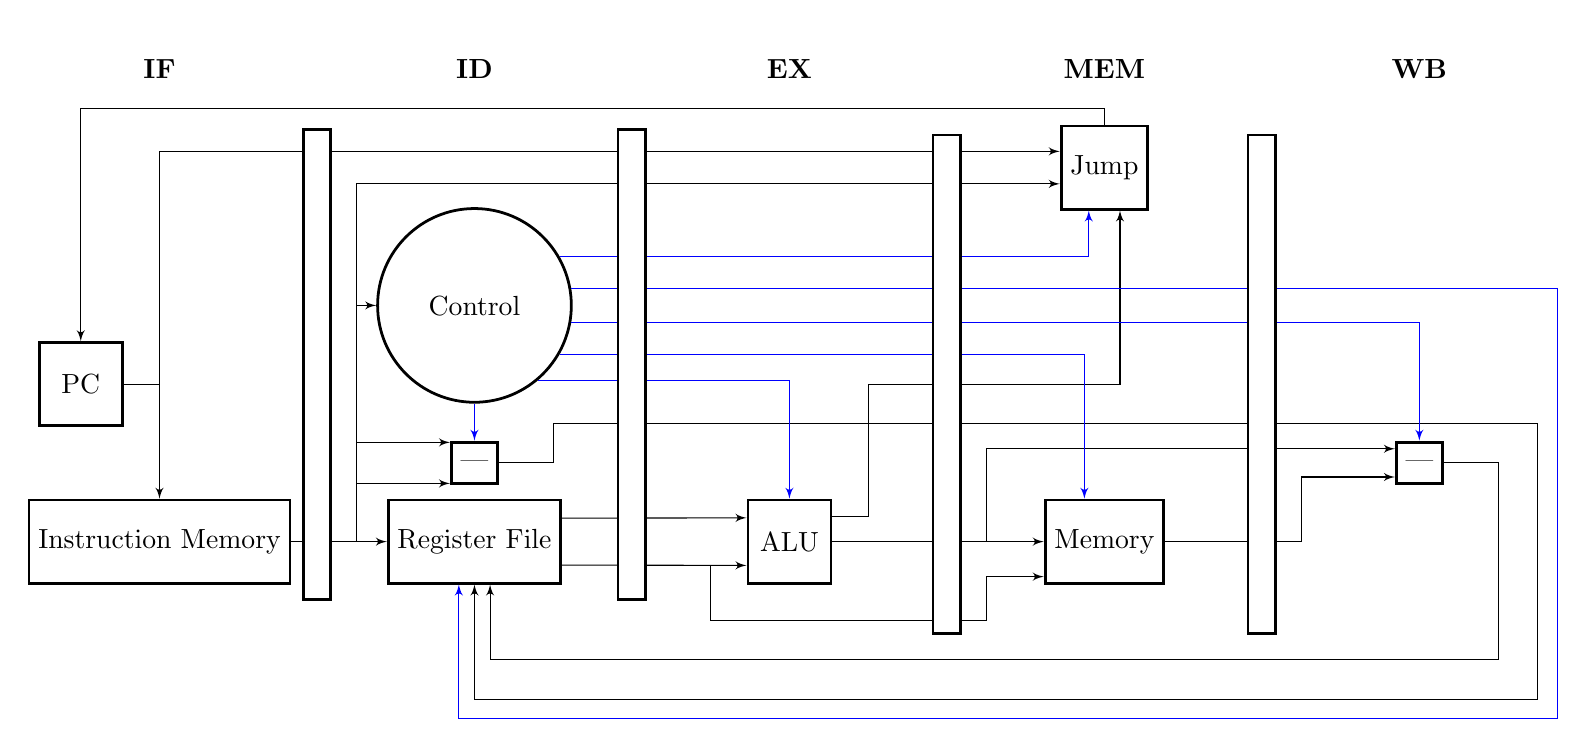
\begin{tikzpicture}
                \node[block] (alu) at (0,0) {ALU};
                \node[block] (reg) at (-4,0) {Register File};
                \node[block] (memo) at (4,0) {Memory};
                \node[block] (jump) at (4,4.75) {Jump};
                \node[block] (imem) at (-8,0) {Instruction Memory};
                \node[block] (pc) at (-9, 2) {PC};
                \node[control] (cont) at (-4, 3) {Control};
                \node[mux] (wbm) at (8,1) {|};
                \node[mux] (addr) at (-4, 1) {|};

                \node[empty] (if) at (-8, 6) {\textbf{IF}};
                \node[empty] (id) at (-4, 6) {\textbf{ID}};
                \node[empty] (ex) at (0, 6) {\textbf{EX}};
                \node[empty] (mem) at (4, 6) {\textbf{MEM}};
                \node[empty] (wb) at (8, 6) {\textbf{WB}};

                \path[draw, ->] (-5.5,0) |- (addr.220);
                \path[draw, ->] (-5.5,0) |- (addr.140);
                \path[draw, ->] (pc) -| (imem);
                \path[draw, ->] (imem) -- (reg);
                \path[draw, ->] (-5.5,0) |- (cont);
                \path[draw, ->] (reg.15) -- (alu.151);
                \path[draw, ->] (reg.345) -- (alu.209);
                \path[draw, ->] (alu) -- (memo);
                \path[draw, ->] (-1,-0.31) -| (-1,-1) -- (2.5,-1) |- (memo.210);
                \path[draw, ->] (2.5, 0) |- (wbm.150);
                \path[draw, ->] (memo) -- (6.5, 0) |- (wbm.210);
                \path[draw, ->] (wbm) -| (9, -1.5) -| (reg.290);
                \path[draw, ->] (alu.30) -| (1,1) |- (4,2) -| (jump.290);
                \path[draw, ->] (jump) |- (0,5.5) -| (pc);
                \path[draw, ->] (-8,2) |- (jump.160);
                \path[draw, ->] (-5.5,3) |- (jump.200);
                \path[draw, ->] (addr) -| (-3, 1.5) -| (9.5,-2) -|
                (reg.270);

                \path[draw, color=blue, ->] (cont.310) -| (alu);
                \path[draw, color=blue, ->] (cont.330) -| (memo.115);
                \path[draw, color=blue, ->] (cont.350) -| (wbm);
                %\path[draw, color=blue, ->] (cont.10) -| (9.5,-2) -| (reg.250);
                \path[draw, color=blue, ->] (cont.10) -| (9.75,-2.25) -| (reg.250);
                \path[draw, color=blue, ->] (cont.30) -| (jump.250);
                \path[draw, color=blue, ->] (cont) -- (addr);

                \node[block, minimum height=170, minimum width=10, fill=white] (ifid) at
                (-6,2.25) {};
                \node[block, minimum height=170, minimum width=10, fill=white] (idex) at
                (-2,2.25) {};
                \node[block, minimum height=180, minimum width=10, fill=white]
                (exmem) at (2,2) {};
                \node[block, minimum height=180, minimum width=10, fill=white]
                (exmem) at (6,2) {};
            \end{tikzpicture}
        }
        \label{fig:pipes}
    \end{figure}
\end{frame}

\section{Introducing the pipes}
\subsection{Implementation}
\begin{frame}
    We have two ways of implementing pipes in SME:
    \begin{itemize}
        \item Clocked Busses - for busses which only traverses 2 stages
        \item Clocked Processes - for dividing busses traversing more than 2
            stages
    \end{itemize}
    Just adding the \texttt{ClockedBus} attribute to the busses seems simpler.
    However, it can become more explicit, by adding additional busses, and to
    have a process, which explicitly touches all of the busses, which should go
    into the pipe.
\end{frame}
\begin{frame}
    Introducing the pipes is fairly straightforward. For each pipe, we add a
    copy of the bus, which the 'next' stage needs. Then, for each pipe, we add
    an SME process, which takes all the busses from the 'previous' stage, and
    outputs their data on the matching newly added pipe bus. Finally, the
    references in the 'next' stage should be updated to look at the piped
    busses.
\end{frame}
\begin{frame}
    This process can be repeated for all of the required pipes. There is only
    one problem: the Jump Unit. The processor do not know when to jump, until
    the MEM stage, as the adresses needs to be computed in the EX stage.

    \vspace{\baselineskip}
    To solve this, the Jump Unit should be divided out to the different stages.
    The IF stage should handle incrementing the Program Counter, and choosing
    between the addresses from the MEM stage, and the incremented Program
    Counter.

    \vspace{\baselineskip}
    The EX stage should as mentioned, compute the addresses, and finally, the
    MEM stage should hold the logic for choosing between the branch address and
    the jump address.
\end{frame}
\begin{frame}
    Finally, in the single cycle MIPS processor, we added a Write Buffer in
    order to eliminate the cycle from the Register File to the Register File.

    \vspace{\baselineskip}
    However, by introducing pipes, we have also introduced buffers, and as
    such, we can remove the Write Buffer.
\end{frame}

\subsection{Testing}
\begin{frame}
    To test the pipelined processor, we could use any of the programs we have
    previously written. However, since we have pipelined the processor, we
    need to insert bubbles in our program, to ensure the data is ready for all
    of the instructions.

    \vspace{\baselineskip}
    An bubble is a No Operation (\texttt{nop}) instruction, which performs no
    operation, and touches neither the Register File nor the Memory.
\end{frame}
\begin{frame}
    We are going to implement a simple program, which is easy to verify: a
    small loop, which computes $n$ fibonacci numbers, and places them in
    memory.

    \vspace{\baselineskip}
    As we have done previously, we are going to give pseudo low level C code.
\end{frame}
\begin{frame}[fragile]
\begin{lstlisting}
void init(int *arr) {
    *(arr)   = 1;
    *(arr+1) = 1;
}

void loop(int *arr, int n) {
    int i, tmp1, tmp2, tmp3;
    for (i = 0; i < n; i++) {
        tmp1 = *(arr+i);
        tmp2 = *(arr+i+1);
        tmp3 = tmp1 + tmp2;
        *(arr+i+2) = tmp3;
    }
}
\end{lstlisting}
\end{frame}
\begin{frame}
    Note: if the program is written in actual C, the allocated array should be
    $n+2$, due to initialization values.

    \vspace{\baselineskip}
    Furthermore, when we port it to MIPS assembly, after each instruction, we
    should insert a bubble of 4 \texttt{nop}'s.

    \vspace{\baselineskip}
    When the program has run, the $n+2$ fibonacci numbers should be in memory,
    at the given address.
\end{frame}

\section{Forwarding}
\begin{frame}
    By introducing pipes, we also introduced data hazards and control hazards.
    We start by looking at handling data hazards.

    \vspace{\baselineskip}
    Data hazards are when one instruction writes to a register that a following
    instruction reads from. This was not a problem in the single cycle
    processor, as all the data had been written in the same clock cycle.
\end{frame}
\begin{frame}
    We can eliminate some of the data hazards by implementing an additional
    unit: the Forwarding Unit.

    \vspace{\baselineskip}
    This unit looks at the registers used by the instruction in the EX stage,
    and if the instruction in either the MEM or the WB stage writes to either
    of the registers, then the Forwarding will forward that data to the EX
    stage.
\end{frame}
\begin{frame}
    \begin{figure}
        \centering
        \scalebox{0.5}{
            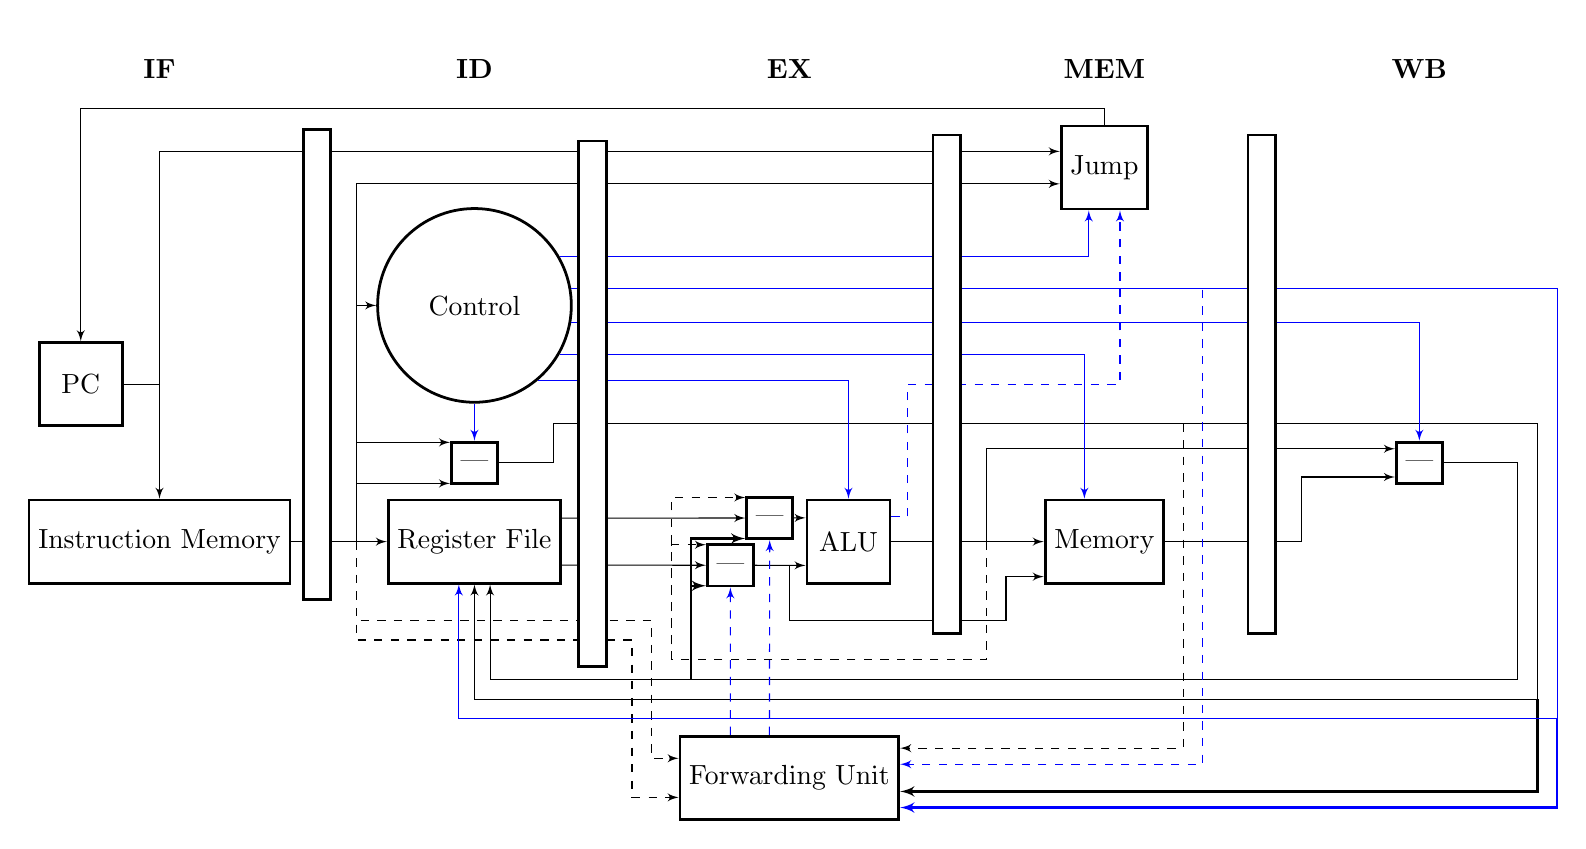
\begin{tikzpicture}
                \node[block] (alu) at (0.75,0) {ALU};
                \node[block] (reg) at (-4,0) {Register File};
                \node[block] (memo) at (4,0) {Memory};
                \node[block] (jump) at (4,4.75) {Jump};
                \node[block] (imem) at (-8,0) {Instruction Memory};
                \node[block] (pc) at (-9, 2) {PC};
                \node[control] (cont) at (-4, 3) {Control};
                \node[mux] (wbm) at (8,1) {|};
                \node[block] (forw) at (0, -3) {Forwarding Unit};
                \node[mux] (forwa) at (-0.25, 0.3) {|};
                \node[mux] (forwb) at (-0.75, -0.3) {|};
                \node[mux] (addr) at (-4, 1) {|};

                \node[empty] (if) at (-8, 6) {\textbf{IF}};
                \node[empty] (id) at (-4, 6) {\textbf{ID}};
                \node[empty] (ex) at (0, 6) {\textbf{EX}};
                \node[empty] (mem) at (4, 6) {\textbf{MEM}};
                \node[empty] (wb) at (8, 6) {\textbf{WB}};

                \path[draw, ->] (pc) -| (imem);
                \path[draw, ->] (imem) -- (reg);
                \path[draw, ->] (-5.5,0) |- (cont);
                \path[draw, ->] (-5.5,0) |- (addr.220);
                \path[draw, ->] (-5.5,0) |- (addr.140);
                %\path[draw, ->] (reg.15) -- (alu.151);
                \path[draw, ->] (reg.15) -- (forwa);
                \path[draw, ->] (forwa) --  (alu.151);
                \path[draw, ->] (reg.345) -- (forwb);
                \path[draw, ->] (forwb) -- (alu.209);
                \path[draw, ->] (alu) -- (memo);
                \path[draw, ->] (0,-0.3) |- (0,-1) -- (2.75,-1) |- (memo.210);
                \path[draw, ->] (2.5, 0) |- (wbm.150);
                \path[draw, ->] (memo) -- (6.5, 0) |- (wbm.210);
                \path[draw, ->] (wbm) -| (9.25, -1.75) -| (reg.290);
                \path[draw, color=blue, dashed, ->] (alu.30) -| (1.5,1) |- (4,2) -| (jump.290);
                \path[draw, ->] (jump) |- (0,5.5) -| (pc);
                \path[draw, ->] (-8,2) |- (jump.160);
                \path[draw, ->] (-5.5,3) |- (jump.200);
                \path[draw, thick, ->] (-1.25,-1.75) |- (forwb.220);
                \path[draw, thick, ->] (-1.25,-1.75) |- (forwa.220);
                \path[draw, dashed, ->] (2.5, 0) |- (-1.5, -1.5) |- (forwb.140);
                \path[draw, dashed, ->] (-1.5, -1.5) |- (forwa.140);
                \path[draw, ->] (addr) -| (-3, 1.5) -| (9.5,-2) -|
                (reg.270);
                \path[draw, thick, ->] (9.5, -2) |- (forw.353);
                \path[draw, dashed, ->] (5,1.5) |- (forw.15);
                \path[draw, dashed, ->] (-5.5,0) |- (-1.75,-1) |- (forw.170);
                \path[draw, dashed, ->] (-5.5,0) |- (-2,-1.25) |- (forw.190);

                \path[draw, color=blue, ->] (cont.310) -| (alu);
                \path[draw, color=blue, ->] (cont.330) -| (memo.115);
                \path[draw, color=blue, ->] (cont.350) -| (wbm);
                \path[draw, color=blue, ->] (cont.10) -| (9.75,-2.25) -| (reg.250);
                \path[draw, color=blue, ->] (cont.30) -| (jump.250);
                \path[draw, color=blue, ->] (cont) -- (addr);
                \path[draw, color=blue, thick, ->] (9.75,-2.25) |- (forw.345);
                \path[draw, color=blue, dashed, ->] (5.25, 3.2) |- (forw.7);

                \path[draw, color=blue, dashed, ->] (forw.115) -- (forwa);
                \path[draw, color=blue, dashed, ->] (forw.144) -- (forwb);


                \node[block, minimum height=170, minimum width=10, fill=white] (ifid) at
                (-6,2.25) {};
                \node[block, minimum height=190, minimum width=10, fill=white] (idex) at
                (-2.5,1.75) {};
                \node[block, minimum height=180, minimum width=10, fill=white]
                (exmem) at (2,2) {};
                \node[block, minimum height=180, minimum width=10, fill=white]
                (exmem) at (6,2) {};
            \end{tikzpicture}
        }
        \label{fig:forw}
    \end{figure}
\end{frame}

\subsection{Implementation \& Testing}
\begin{frame}
    Implementing the Forwarding unit should be done with an SME process, which
    should be put in the EX stage.

    \vspace{\baselineskip}
    The unit should be controlling two multiplexors, which decides whether the
    EX stage should use the values read from registers, the value from the MEM
    stage or the value from the WB stage.

    \vspace{\baselineskip}
    Testing the forwarding unit is straightforward: we just remove the
    \texttt{nop}'s from the fibonacci program, except for those following a
    load, branch or jump, as these hazards are not handled yet.
\end{frame}

\section{Hazard Detection}
\subsection{Data Hazards}
\begin{frame}
    As we just mentioned, we cannot handle all of the data hazards with just
    fowarding. This is due to the forwarding destination being the EX stage,
    and that the data might not be ready at that point.

    \vspace{\baselineskip}
    E.g. if we have a load instruction, which is followed by an instruction
    that uses the loaded data in its computation. In this case, the loaded data
    will not be ready until the load instruction has reached the WB stage.

    \vspace{\baselineskip}
    To handle this, the processor needs to detect the hazard, and insert a
    bubble, and stall some of the pipes and registers.
\end{frame}

\subsection{Control Hazards}
\begin{frame}
    We also need to handle an additional type of hazard: control hazards.
    Control hazards are when either a jump or a branch instruction has been
    executed.

    \vspace{\baselineskip}
    The problem is that the branch or jump is not performed until the MEM
    stage, which means that all of the previous states of the pipeline may have
    been filled with instructions, which should not be executed.

    \vspace{\baselineskip}
    To solve this, we should detect the hazard, and in such case flush the
    pipeline. Flushing is the action of resetting the registers in the pipes,
    so they output \texttt{nop} instructions.
\end{frame}
\begin{frame}
    \begin{figure}
        \centering
        \scalebox{0.5}{
            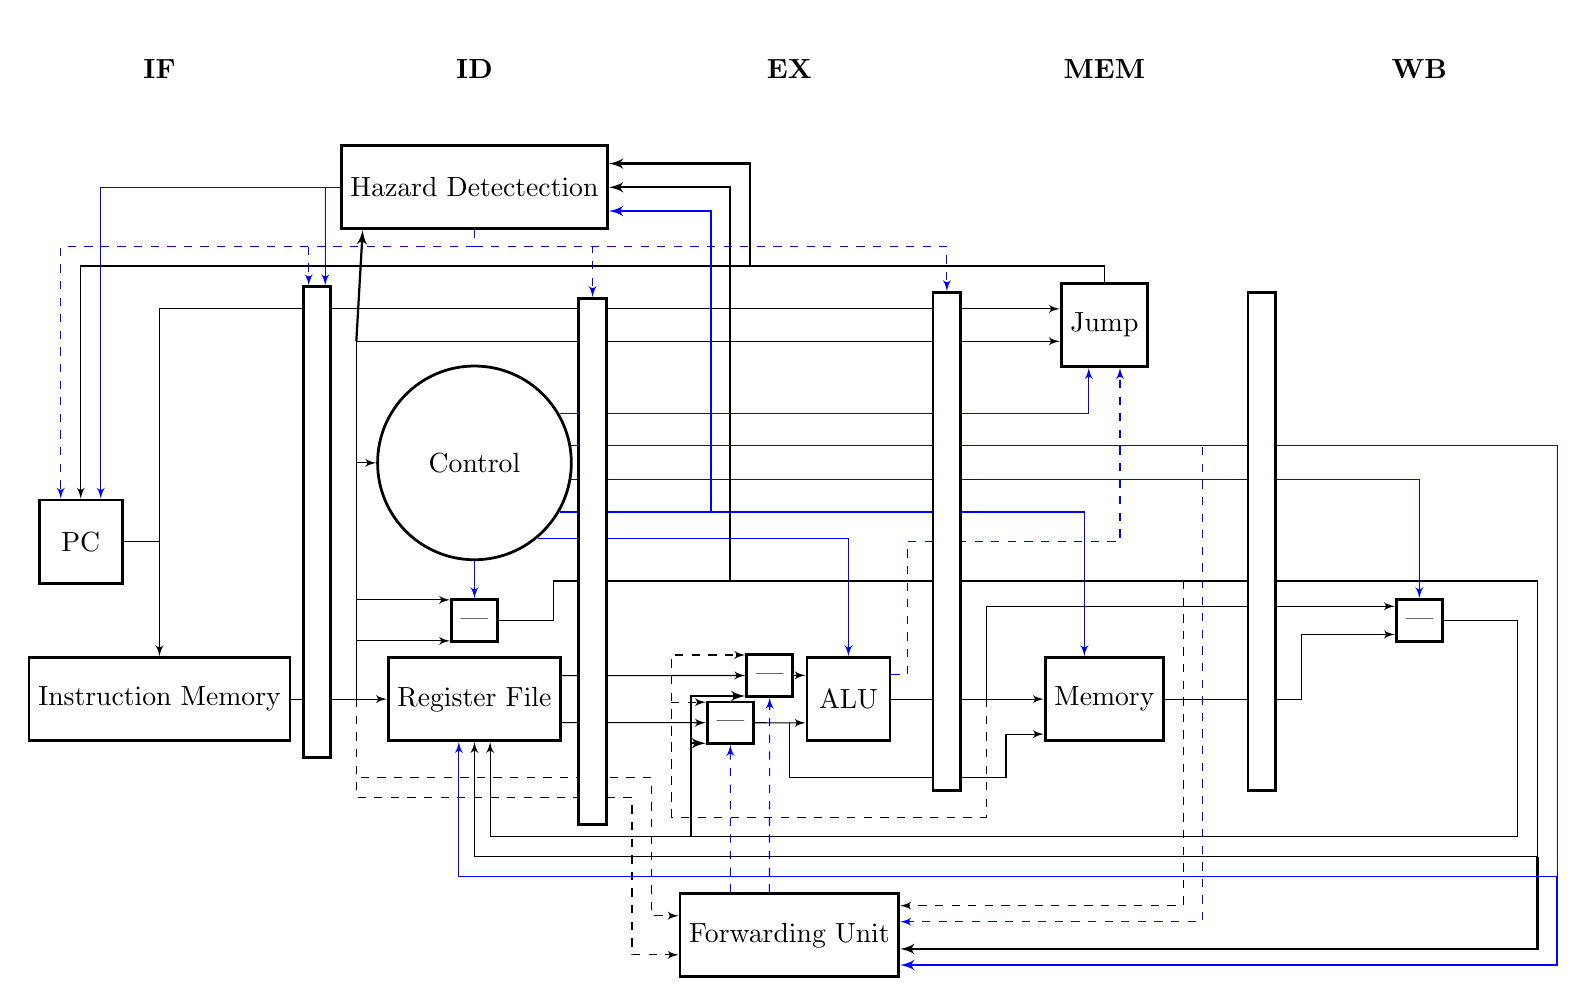
\begin{tikzpicture}
                \node[block] (alu) at (0.75,0) {ALU};
                \node[block] (reg) at (-4,0) {Register File};
                \node[block] (memo) at (4,0) {Memory};
                \node[block] (jump) at (4,4.75) {Jump};
                \node[block] (imem) at (-8,0) {Instruction Memory};
                \node[block] (pc) at (-9, 2) {PC};
                \node[control] (cont) at (-4, 3) {Control};
                \node[mux] (wbm) at (8,1) {|};
                \node[block] (forw) at (0, -3) {Forwarding Unit};
                \node[mux] (forwa) at (-0.25, 0.3) {|};
                \node[mux] (forwb) at (-0.75, -0.3) {|};
                \node[mux] (addr) at (-4, 1) {|};
                \node[block] (haz) at (-4,6.5) {Hazard Detectection};

                \node[empty] (if) at (-8, 8) {\textbf{IF}};
                \node[empty] (id) at (-4, 8) {\textbf{ID}};
                \node[empty] (ex) at (0, 8) {\textbf{EX}};
                \node[empty] (mem) at (4, 8) {\textbf{MEM}};
                \node[empty] (wb) at (8, 8) {\textbf{WB}};

                \path[draw, ->] (pc) -| (imem);
                \path[draw, ->] (imem) -- (reg);
                \path[draw, ->] (-5.5,0) |- (cont);
                \path[draw, ->] (-5.5,0) |- (addr.220);
                \path[draw, ->] (-5.5,0) |- (addr.140);
                %\path[draw, ->] (reg.15) -- (alu.151);
                \path[draw, ->] (reg.15) -- (forwa);
                \path[draw, ->] (forwa) --  (alu.151);
                \path[draw, ->] (reg.345) -- (forwb);
                \path[draw, ->] (forwb) -- (alu.209);
                \path[draw, ->] (alu) -- (memo);
                \path[draw, ->] (0,-0.3) |- (0,-1) -- (2.75,-1) |- (memo.210);
                \path[draw, ->] (2.5, 0) |- (wbm.150);
                \path[draw, ->] (memo) -- (6.5, 0) |- (wbm.210);
                \path[draw, ->] (wbm) -| (9.25, -1.75) -| (reg.290);
                \path[draw, color=blue, dashed, ->] (alu.30) -| (1.5,1) |- (4,2) -| (jump.290);
                \path[draw, ->] (jump) |- (0,5.5) -| (pc);
                \path[draw, ->] (-8,2) |- (jump.160);
                \path[draw, ->] (-5.5,3) |- (jump.200);
                \path[draw, thick, ->] (-1.25,-1.75) |- (forwb.220);
                \path[draw, thick, ->] (-1.25,-1.75) |- (forwa.220);
                \path[draw, dashed, ->] (2.5, 0) |- (-1.5, -1.5) |- (forwb.140);
                \path[draw, dashed, ->] (-1.5, -1.5) |- (forwa.140);
                \path[draw, ->] (addr) -| (-3, 1.5) -| (9.5,-2) -|
                (reg.270);
                \path[draw, thick, ->] (9.5, -2) |- (forw.353);
                \path[draw, dashed, ->] (5,1.5) |- (forw.15);
                \path[draw, dashed, ->] (-5.5,0) |- (-1.75,-1) |- (forw.170);
                \path[draw, dashed, ->] (-5.5,0) |- (-2,-1.25) |- (forw.190);

                \path[draw, color=blue, ->] (cont.310) -| (alu);
                \path[draw, color=blue, ->] (cont.330) -| (memo.115);
                \path[draw, color=blue, ->] (cont.350) -| (wbm);
                \path[draw, color=blue, ->] (cont.10) -| (9.75,-2.25) -| (reg.250);
                \path[draw, color=blue, ->] (cont.30) -| (jump.250);
                \path[draw, color=blue, ->] (cont) -- (addr);
                \path[draw, color=blue, thick, ->] (9.75,-2.25) |- (forw.345);
                \path[draw, color=blue, dashed, ->] (5.25, 3.2) |- (forw.7);

                \path[draw, color=blue, dashed, ->] (forw.115) -- (forwa);
                \path[draw, color=blue, dashed, ->] (forw.144) -- (forwb);

                % Hazard
                \path[draw, thick, ->] (-0.75, 1.5) |- (haz); % addr
                \path[draw, thick, color=blue, ->] (-1, 2.37) |- (haz.350); % mem
                \path[draw, thick, ->] (-0.5, 5.5) |- (haz.10); % pcsrc
                \path[draw, thick, ->] (-5.5, 4.55) -- (haz.201);% reada readb
                \path[draw, dashed, color=blue, -] (haz) -- (-4, 5.75);

                \node[block, minimum height=170, minimum width=10, fill=white] (ifid) at
                (-6,2.25) {};
                \node[block, minimum height=190, minimum width=10, fill=white] (idex) at
                (-2.5,1.75) {};
                \node[block, minimum height=180, minimum width=10, fill=white]
                (exmem) at (2,2) {};
                \node[block, minimum height=180, minimum width=10, fill=white]
                (memwb) at (6,2) {};

                \path[draw, dashed, color=blue, ->] (-4, 5.75) -| (exmem);
                \path[draw, dashed, color=blue, ->] (-4, 5.75) -| (idex);
                \path[draw, dashed, color=blue, ->] (-4, 5.75) -| (ifid.92);
                \path[draw, dashed, color=blue, ->] (-4, 5.75) -| (pc.115);
                \path[draw, color=blue, ->] (haz) -| (ifid.88);
                \path[draw, color=blue, ->] (haz) -| (pc.65);
            \end{tikzpicture}
        }
        \label{fig:hazard}
    \end{figure}
\end{frame}

\subsection{Implementation}
\begin{frame}
    The Hazard Detection Unit should be implemented in its own SME process.

    \vspace{\baselineskip}
    To handle the data hazards, the process should read the \texttt{memread}
    flag from the EX stage, the destination register from the EX stage, and the
    two source register address from the ID stage. If the flag has been set,
    and the destination address match either of the two source adddresses, the
    ID/EX pipe should be flushed, the IF/ID and the PC register should be
    stalled.

    \vspace{\baselineskip}
    Stalling is setting the registers not to update, so they will output the
    same data in the next clock cycle.
\end{frame}
\begin{frame}
    To solve the control hazards, the unit should look at the signal from the
    MEM stage, which indicates whether or not jumping should be performed.

    \vspace{\baselineskip}
    In such a case, the Hazard Detection Unit should send a signal to flush the
    IF/ID, ID/EX and EX/MEM pipes. Note: the PC register should perform
    normally, even though it might have been instructed to stall, as the stall
    is now invalid.
\end{frame}

\subsection{Testing}
\begin{frame}
    Testing this is straightforward, as the processor should be able to handle
    all of our previous programs, albeit with more clock cycles.

    \vspace{\baselineskip}
    Note: if these programs are tested against the single cycle processor, the
    performance will be worse, when simulating. This is due to more processes
    and busses, which gives the simulation more work. There should not be any
    performance hit, when the processor is run on hardware.
\end{frame}

% exit section
\AtBeginSection{}
\section*{}

% {{{ Bibliography ------------------------------------------------------------
%\begin{frame}{Bibliography}
%  \tiny
%  \bibliographystyle{plain}
%  \bibliography{pl}
%\end{frame}
% }}} -------------------------------------------------------------------------

\end{document}
